\section{Malonic Acid Orientation}

Our discussion of the molecular orientation of malonic acid begins with a be description of the angles used in the following analysis. Because the carbon atoms form the backbone of the malonic acid molecular structure, determining the orientation of the three atoms is the first step in understanding the overall orientation of the molecule in space with respect to a water surface.  We describe the orientation of the carbon chain backbone using two angles, and we orient the molecule internally using two dihedral angles.  All the angle definitions described here are depicted in Figure \ref{fig:angle-definitions}. 

The group of three carbon atoms forms a moiety with a $C_{2v}$ symmetry.  The two C-C bond vectors have a bisector between them.  In this work we always refer to the bisector as a vector pointing out from the central carbon in the direction of the other two carbon atoms.  The first angle we define, $\theta$, describes the ``tilt'' of the triatomic carbon chain that forms the acid's backbone. The angle $\theta$ is calculated as the angle formed between the carbon group bisector vector and a reference axis oriented perpendicularly to the water surface, pointing out of the water bulk towards the gas phase side of the water interface. When $\theta = 0$\textdegree, the bisector vector aligns with the reference axis. A value of $\theta=90$\textdegree~places the bisector vector in the plane of the water surface, perpendicular to the reference axis. Rotating the bisector to $\theta=180$\textdegree~makes the bisector anti-aligned with the reference axis, pointing in towards the water side of the interface.

The second angle used to orient the malonic acid carbon backbone, $\phi$, describes a molecular ``twist'' of the malonic acid. This twist angle is defined as a rotation of the plane formed by the three carbon atoms around the bisector axis. For different orientations of the angle $\theta$, the distribution of $\phi$ will necessarily become isotropic because of the symmetries of the plane of the aqueous slab surface. However, the value of $\phi$ is necessary to describe the overall molecular orientation for $\theta$ values near 90\textdegree. When $\theta = 90$\textdegree, the bisector of the carbon atom group lays parallel to the water surface. In such a configuration, $\phi = 0$\textdegree~means the plane of the carbon atoms orients perpendicularly to the plane of the water surface. Likewise, $\phi=90$\textdegree~lays the plane of the carbon atom group flat on the surface, parallel to the plane of the water interface.

\begin{figure}[h!]
	\begin{center}
		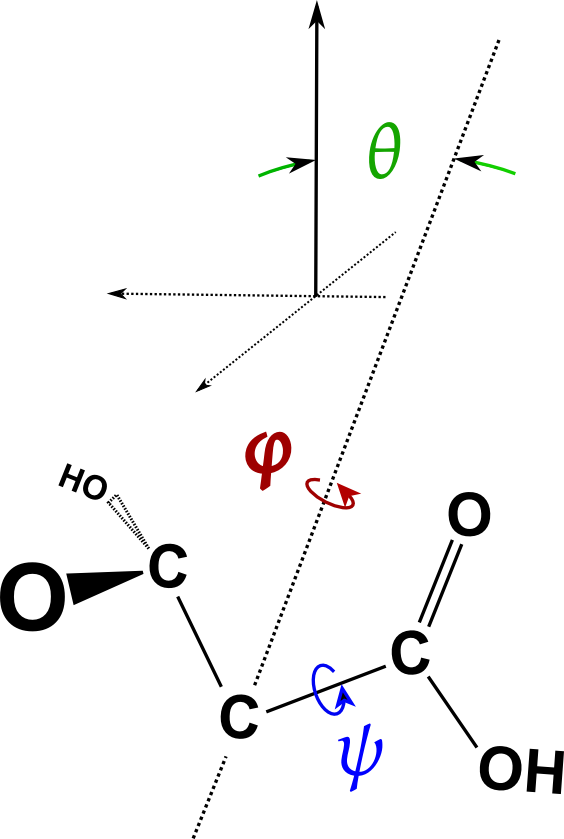
\includegraphics[scale=1.0]{images/malonic-angles/malonic-angles.png}
		\caption{Several angles are used to orient a malonic acid molecule both in the space-fixed frame, and internally in the molecular frame. The carbon backbone of the acid molecule has a $C_{2v}$ symmetry with a central bisector axis splitting the two C-C bonds. The bisector axis ``tilts'' relative to a fixed reference axis to form the angle $\theta$ (green). A rotation of the carbon chain group about the bisector axis changes the ``twist'' angle, $\phi$ (red). The carboxylic acid groups can orient by a rotation about the two C-C bonds. The dihedral angles, $\psi$ (blue/purple), set the internal molecular orientation of the the two carboxylic acid groups. $\psi=0$\textdegree~when a carboxylic acid is rotated such that the plane formed by the O=C-O is parallel to the plane of the three carbons, and the carbonyl C=O bond points in the direction of the carbon chain bisector. Two values of $\psi$ are depicted (right) to show how the carboxylic acid group rotates within the acid molecule.}
		\label{fig:angle-definitions}
	\end{center}
\end{figure}

The planes formed by the atoms of the carboxylic acid groups orient by rotation of two dihedral angles, $\psi$, referenced to the plane of the three backbone carbon atoms. The dihedral angle $\psi$ is the angle of rotation of the C-C bond between the central methylene carbon, and a carbonyl carbon of a carboxylic acid moiety. The reference orientation that sets $\psi=0$\textdegree~is defined by two conditions: 1) the plane of the atoms of the carboxylic acid orients parallel to the plane of the three carbon atoms, and 2) the carbonyl C=O bond vector (pointing from the C to the O) points to the same side as the C-C-C bisector vector (i.e. $\overline{C=O} \cdot \overline{bisector} > 0$). A dihedral angle of $\psi=90$\textdegree~rotates the O=C-O plane perpendicular to the C-C-C plane. Lastly, $\psi=180$\textdegree~rotates the carboxylic acid such that the carbonyl is anti-aligned with the C-C-C bisector. The various orientations of the dihedral angles are depicted in Figure \ref{fig:angle-definitions}, and characterize the internal orientation of malonic acid. By combining all four of the described angles with information about the acid position we are able to develop a nearly complete picture of the orientational behavior of malonic acid relative to a nearby water surface.


\subsection {Carbon Backbone Orientation}

Bivariate angle distributions of $\theta$ and $\phi$ were calculated for the three carbon backbone atoms, and are shown in Figure \ref{fig:backbone-theta-phi}. The set of plots represents slices through the interface. Each slice is located at the distance labeled in the top-right of the respective plot. Positive positions are further into the vacuum phase, and negative positions are further into the water side of the interface. A distance of 0\angs~is located at the water surface location. The location of the surface, and all calculations performed to relate interfacial position are done using a method of averaging top-most water molecule positions, and is fully described in our previous publication.\cite{Shamay2011}

In each set of axes of Figure \ref{fig:backbone-theta-phi}, the values of $\theta$ and $\phi$ are plotted along the horizontal and vertical axes, respectively. The plots are two-dimensional histograms colored by the intensity (i.e. population) of the respective location in the angle space. Higher intensity is colored in dark red, and lower intensity is dark blue. Areas in the plots characterized by uniform coloration indicate an isotropic distribution of angles. A concentrated region of distinct coloration indicates an orientational preference in one or both of the angular degrees of freedom.

\begin{figure}[h!]
	\begin{center}
		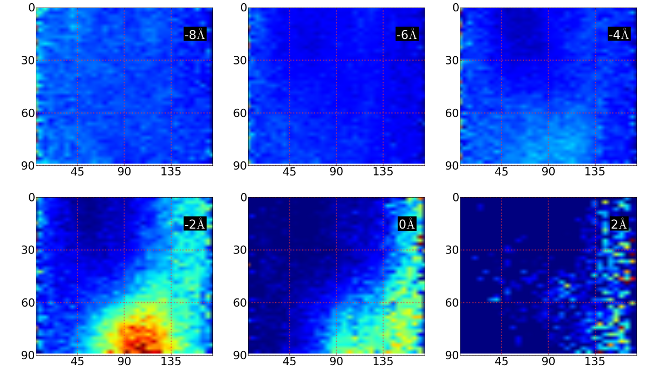
\includegraphics[scale=1.0]{images/malonic-angles/carbonbackbone-theta-phi.png}
		\caption{The overall orientation of a malonic acid molecule in a space-fixed reference frame is determined by the angles $\theta$ and $\phi$ (depicted in Figure \ref{fig:angle-definitions}). The set of plots show the bivariate distribution of the ``tilt'' and ``twist'' of the malonic acid carbon chain, with $\theta$ and $\phi$ values plotted on the horizontal and vertical axes, respectively. Each plot represents a 2\angs~slice of the simulated aqueous slab at a depth listed in the upper-right of the plot.}
		\label{fig:backbone-theta-phi}
	\end{center}
\end{figure}

The plot at a position of 2\angs~shows the orientation of acid molecules just above the water surface, and are most likely less solvated than those further in to the water bulk. The most distinguishing feature is the vertically-running band of intensity to the right of the plot centered between 135\textdegree~and 180\textdegree. This results from a population of acid molecules with their three carbon atoms oriented with the bisector vector pointed more than 45\textdegree~into the water bulk. $\phi$ is spread nearly isotropically in this distribution. However, due to the symmetry of the $\theta$ angle as a spherical coordinate (i.e. a single $\theta$ value describes a cone in space) $\phi$ will necessarily become more isotropic relative to the interface, or spread out across the two-dimensional plots, as $\theta$ takes values near its extrema. $\theta$ values closer to 90\textdegree~require $\phi$ to fully describe the orientation.

A trend in the orientation of the carbon atoms begins at the water surface and below (i.e. $<0$\angs). A second population of acid orientations forms, manifested in the plots as a peak centered at $\theta=90$\textdegree, with $\phi$ also concentrated towards 90\textdegree. This indicates a carbon atom group lying flat in the plane of the water surface. Additionally, as the depth of the molecules increases from 0\angs~to -4\angs, the population above $\theta=135$\textdegree~decreases, and the distribution spreads out both in $\theta$ and in $\phi$. As an acid molecule moves further into the water bulk, and is likely further solvated, the orientational freedom expands in $\theta$ and $\phi$, until at -6\angs~there is a loss of orientational preference, resulting in a flat distribution, and isotropy of the carbon backbone group orientation.

At -4\angs~the $\theta$ distribution expands below $\theta=45$\textdegree. This is due to a population of submerged malonic acid molecules with their bisectors aimed slightly up towards the water surface. Thus we establish that the effect of the phase transition from gas to water bulk, and the field of the interface extends both above and below the water surface with a depth of at least 4\angs~into the water bulk.


\subsection {$CH_2$ Orientation}

The carbon backbone $\theta$ orientation has a strong effect on the orientation of the methylene hydrogens of the acid. An orientation of $\theta=90$\textdegree~aligns the two hydrogens symmetrically above and below the plane of the water interface. At this orientation of $\theta$, as the carbon chain $\phi$ changes, the plane formed by the H-C-H rotates from perpendicular to flat with the water surface. In all orientations centered at $\theta=90$\textdegree~the component of each methylene C-H bond perpendicular to the water surface exactly matches that of the other C-H bond, but in the opposite direction mirrored across the water surface. Furthermore, if the $\theta$ distribution is symmetrically distributed around $\theta=90$\textdegree (as in the -2\angs~plot of Figure \ref{fig:backbone-theta-phi}), then the perpendicular components of the two methylene C-H bonds negate each other. The carbon group $\theta-\phi$ distributions at or below the water surface ($\le 0$\angs) exhibit this quality. Our VSFG experiments failed to produce any spectral features related to the methylene $CH_2$ modes of malonic acid. We propose that this orientational symmetry of the methylene C-H bonds about the water surface manifests spectrally in our polarized VSFG experiments as a lack of intensity where the C-H bond features are expected. 

\subsection {Carbon Backbone Dihedral Angles}

Having established the orientation of the carbon backbone atom group from the $\theta-\phi$ distributions of Figure \ref{fig:backbone-theta-phi}, we now turn to analysis of the  internal geometry of malonic acid carboxylic acid groups near the water surface. The two carboxylic acid moieties rotate around the two C-C bonds, quantified by the two dihedral angles. The magnitudes of the dihedral angles fall in the range 0\textdegree$\le \psi \le$180\textdegree. The O=C-O atomic plane is parallel to the C-C-C plane at $\psi=0$\textdegree~and $\psi=180$\textdegree, and the two planes are perpendicular at $\psi=90$\textdegree, as discussed above and depicted in Figure \ref{fig:angle-definitions}. The two dihedral angles are plotted in a set of bivariate distributions in Figure \ref{fig:carboxylic-psi-psi}. The arrangement of the axes in the figure is identical to that of Figure \ref{fig:backbone-theta-phi}, but with each axis representing one of the two $\psi$ angles.

Figure \ref{fig:carboxylic-psi-psi} shows that the dihedral orientations are strongly related with a preferred rotation of 90\textdegree~apart from each other. The two very concentrated peaks in the plots are located at $\psi=0$\textdegree~and $\psi=90$\textdegree. This results from the carboxylic O=C-O atomic planes of the two carboxylic acids aligning perpendicularly to each other. The topmost plot at 2\angs~is not symmetric between the two dihedral angles with only a single peak in the distribution (located at the left-center of the axis). This is an artifact of how the carboxylic acid groups were distinguished computationally, and indicates that the top-most malonic acids above the water surface take on a fixed dihedral orientation, rarely switching values (i.e. rotating the molecule to flip the alignment of both carboxylic acid groups).


\begin{figure}[h!]
	\begin{center}
		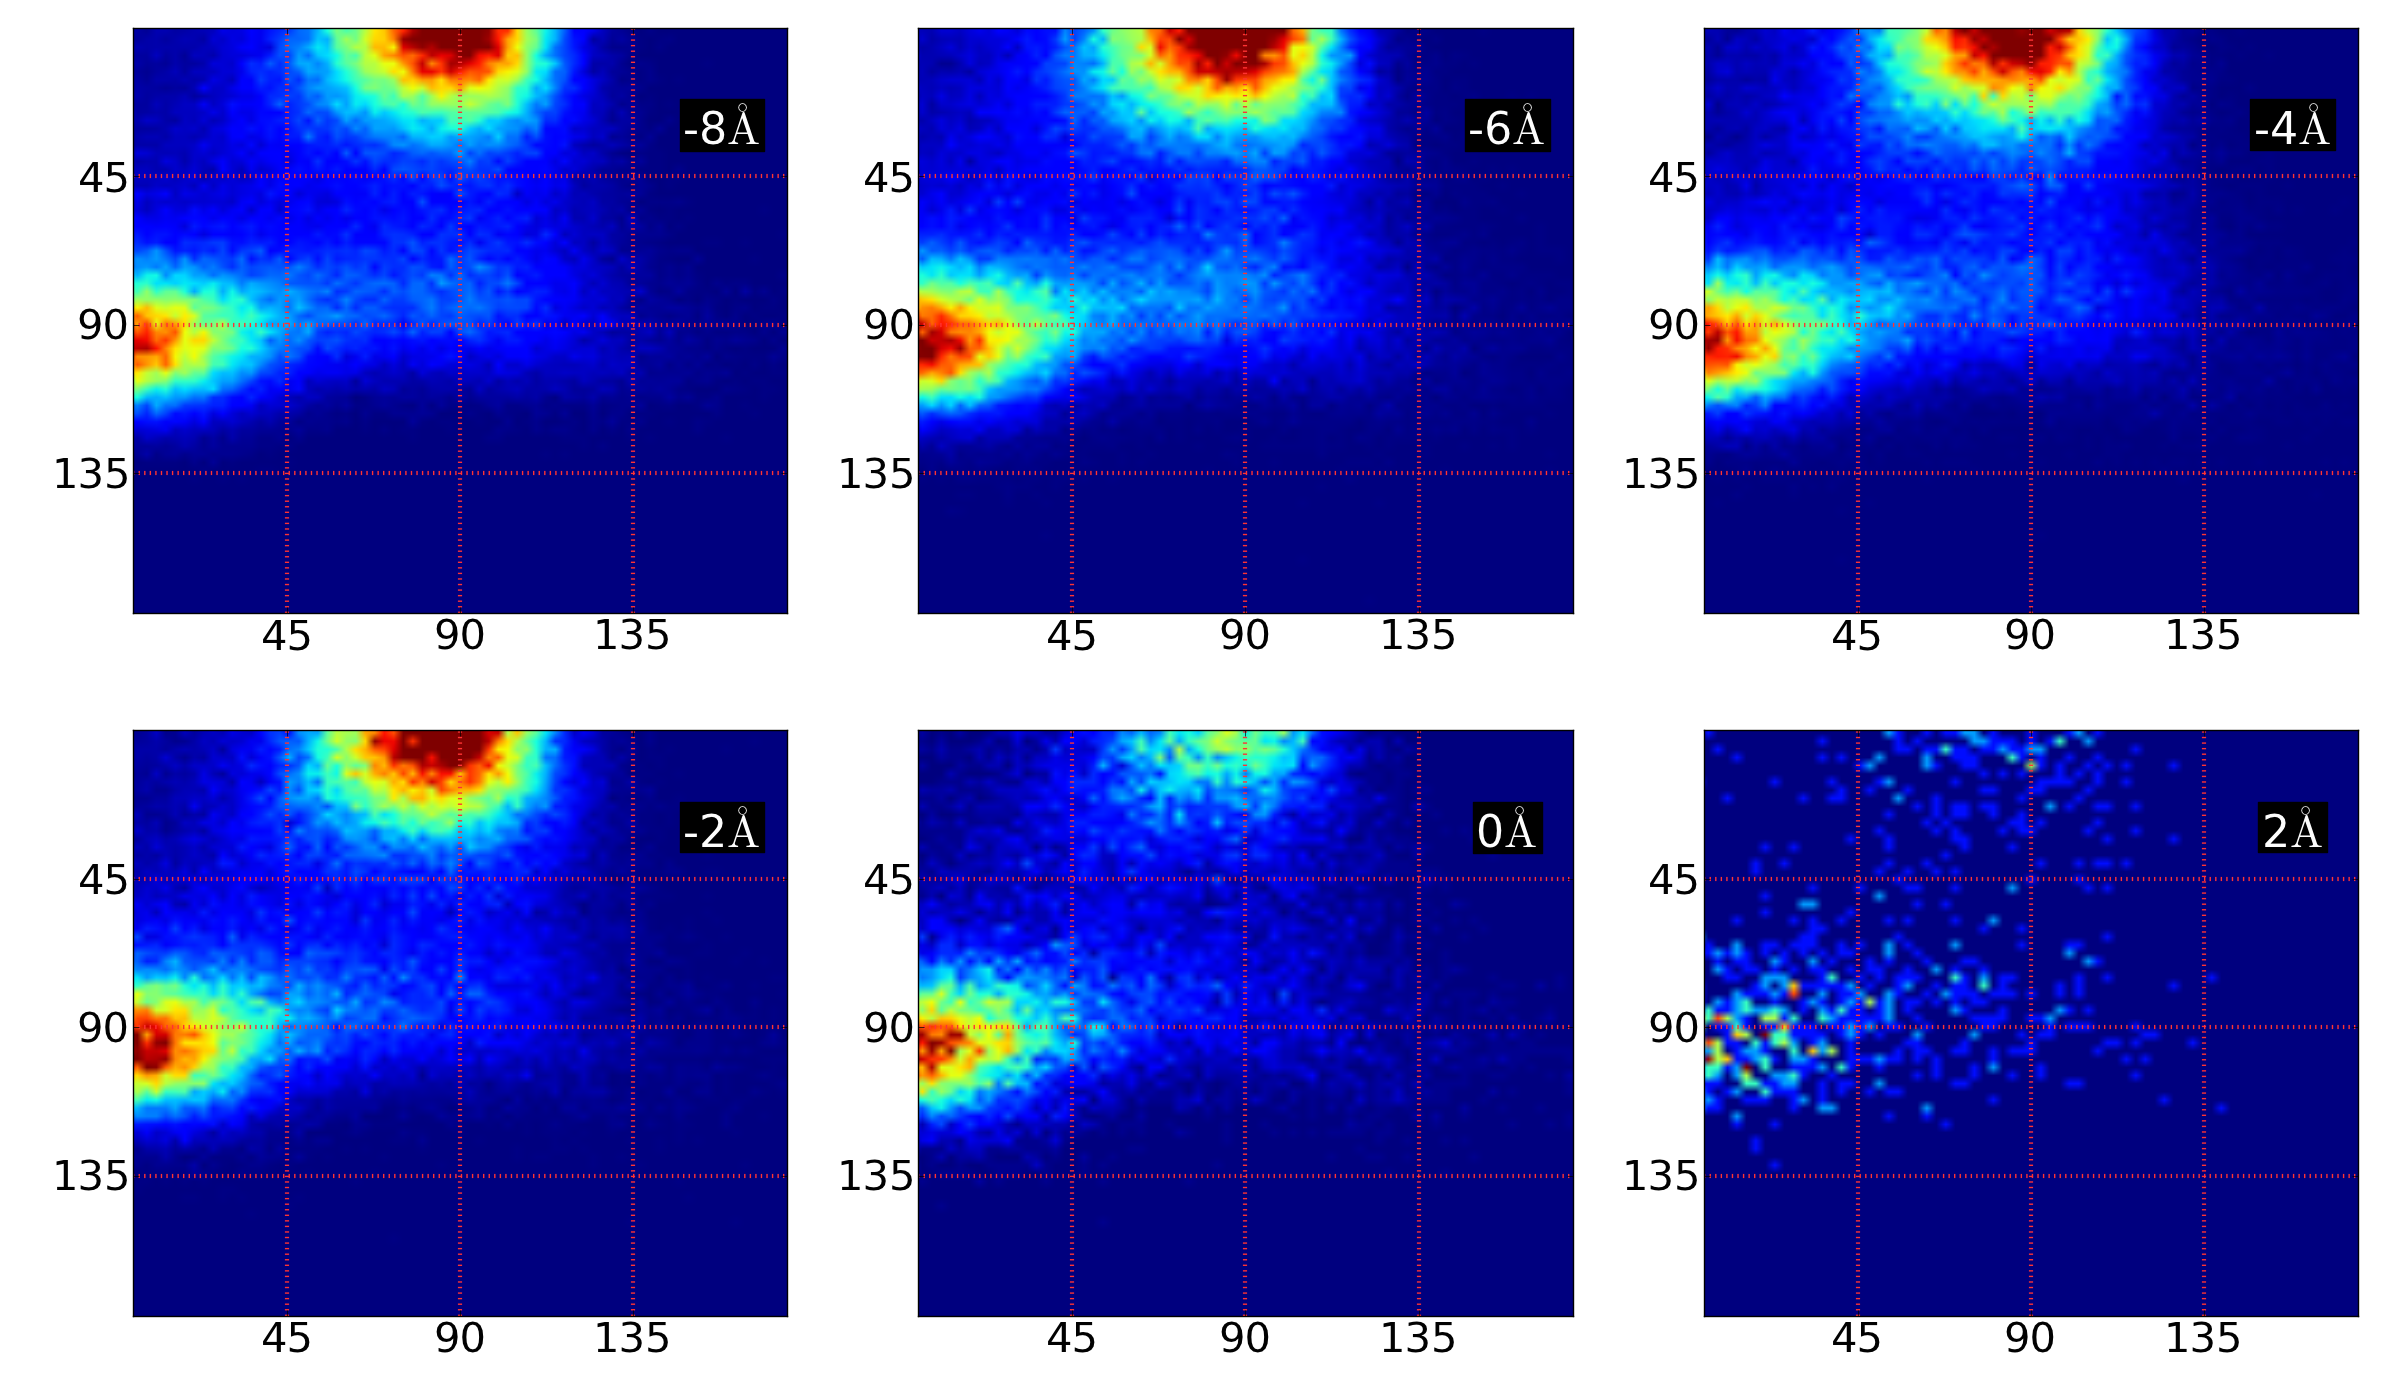
\includegraphics[scale=1.0]{images/malonic-angles/carboxylic-psi-psi.png}
		\caption{Internal orientation of malonic acid is determined here as a function of the dihedral angles, $\psi$. The dihedrals describe the angle formed between the plane of the O=C-O atoms of the carboxylic acid group  and the plane of the three carbon atoms. Orientation of the acid groups changes by rotation around one of the C-C bonds. The reference angle $\psi=0$\textdegree~aligns the carbonyl C=O bond vector parallel to, and in the same direction as the bisector of the carbon chain group. The angles and bond vectors are depicted in Figure \ref{fig:angle-definitions}}
		\label{fig:carboxylic-psi-psi}
	\end{center}
\end{figure}

One of the carbonyl C=O bonds is preferrentially aligned in the same direction as the carbon group bisector ($\psi=0$\textdegree), and in the plane of the plane of the three carbons. The other carbonyl C=O bond points perpendicular to the plane of the carbon group atoms. The strong orientational preference is established both in the bulk of the water and at the water surface location.

There remains one final set of orientational data necessary to fully characterize the interfacial malonic acid. The $\theta-\phi$ distributions of the carbon atoms show that the acid carbon chain lays flat when at the water surface (0\angs), and tilts with the bisector pointing further into the water bulk when the malonic acid is slightly above the water surface. The $\psi-\psi$ dihedral distributions show one C=O carbonyl bond mostly aligned with the carbon group bisector and the other carbonyl aligned normal plane of the carbon atoms. The question remains as to which direction does the perpendicular cabonyl C=O bond vector point? Is it pointed into the water side of the interface, or does it point out towards the gas phase away from the water bulk?

To determine the carbonyl orientation we calculated the tilt angle of the C=O bond, $\theta_{C=O}$. Like the carbon group bisector tilt angle, $\theta_{C=O}$ is referenced to the axis normal to the plane of the water surface, pointing out towards the gas phase side of the interface.

Figure \ref{fig:carbonyl-tilt} shows the angle distribution of $\theta_{C=O}$ plotted as a function of the malonic acid molecular center of mass position. Most of the distribution is isotropic in the tilt angle up to positions several \angs~beneath the water surface location.

Starting above the surface (positions $>0$\angs), the distribution bifurcates into two distinct angle regions. There is a protrusion in the distribution beginning just below 0\angs~and extending above the surface, centered at $\theta_{C=O}=90$\textdegree. A second peak in the distribution is concentrated towards the bottom of the plot near $\theta_{C=O}=180$\textdegree. At this position slightly above the water surface, it is more clear that one of the carbonyl C=O bonds points into the water (the bond oriented near $\theta_{C=O}=180$\textdegree), and the other points more out into the plane of the surface and often slightly angled out from the water phase.  When these two angles are manifested by malonic acid carbonyl bonds just above the water surface, this may lead to a difference in solvation between the two bonds. One bond, pointing more towards the water bulk, will likely have more water interactions than the other that points parallel to, or away from the water surface into the gas phase.


\begin{figure}[h!]
	\begin{center}
		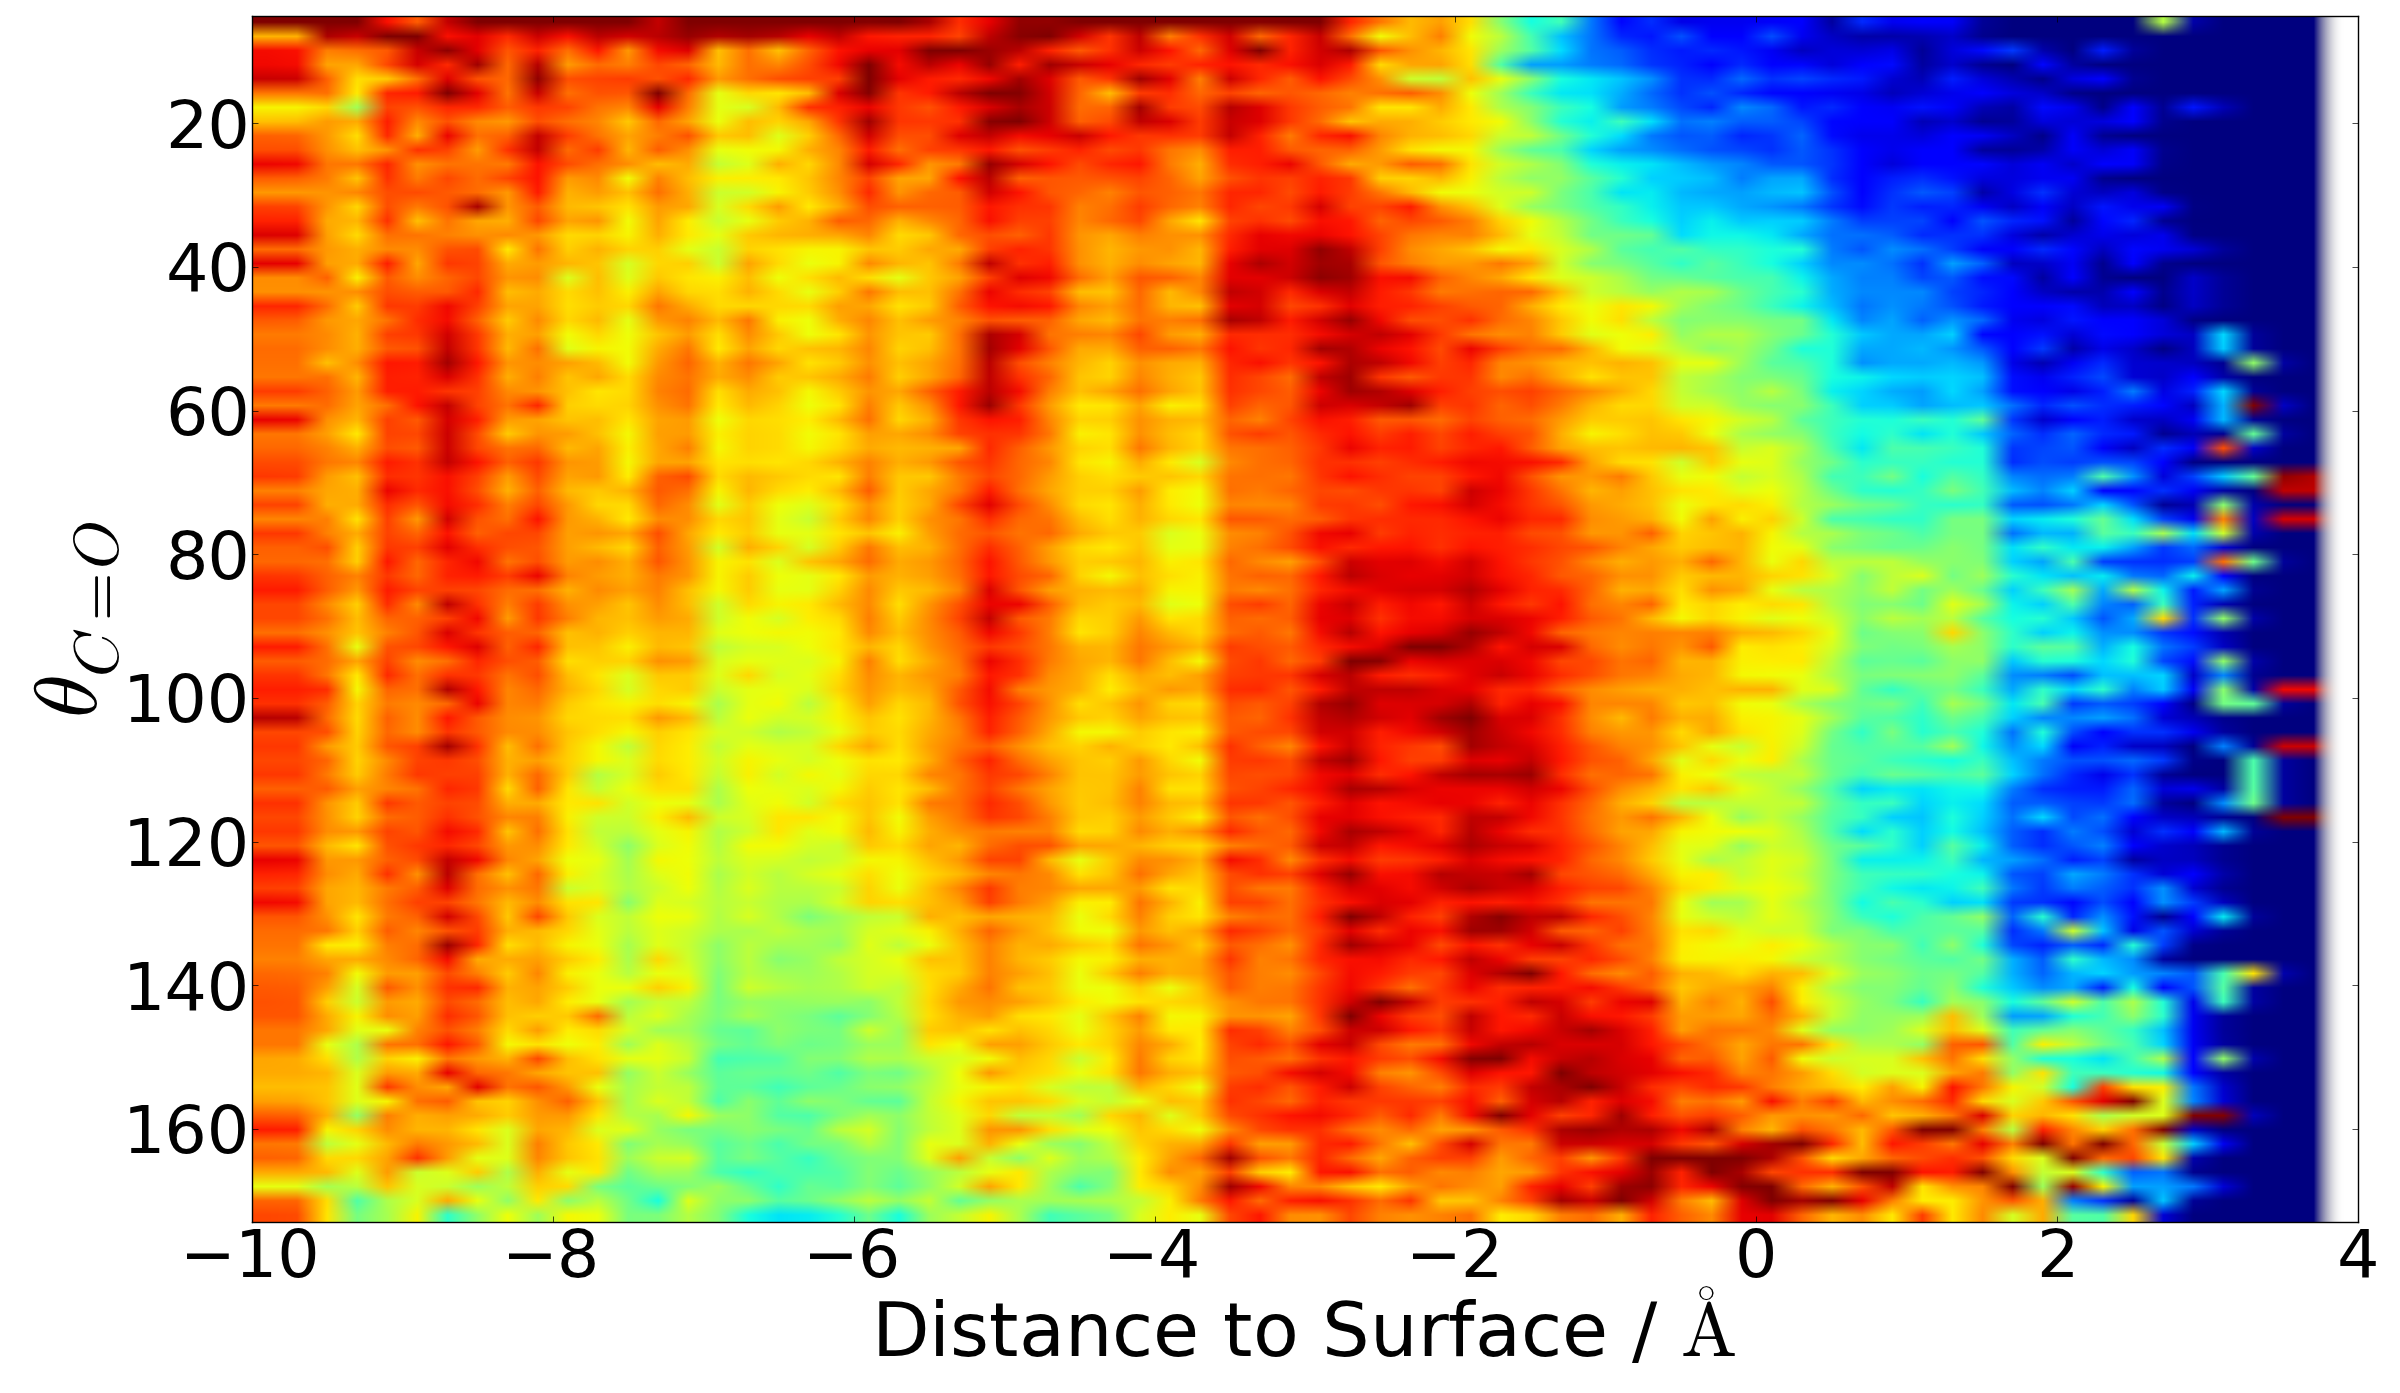
\includegraphics[scale=1.0]{images/malonic-angles/carbonyl-theta-distance.png}
		\caption{Orientation of the carbonyl C=O bonds of both carboxylic acid groups changes with depth in the aqueous interface. Shown is a two-dimensional histogram of the carbonyl bond tilt angle, $\theta_{C=O}$ (vertical axis), plotted against the molecular center of mass position (horizontal axis).}  
		\label{fig:carbonyl-tilt}
	\end{center}
\end{figure}

Further down into the water surface, the angle distribution spreads over a much larger range until becoming isotropic near -2\angs. However, a feature appears at -3\angs~and extends down slightly past -8\angs into the water phase. In this region there is a decreased intensity in the histogram for $\theta_{C=O} > 120$\textdegree. This shows a population of malonic acid carbonyl C=O bonds pointing less into the water bulk below. At this depth, the carbon backbone orientation distribution becomes somewhat more isotropic, but there remains a population of acids with $\theta_{CCC} < 90$\textdegree~(i.e. the carbon group bisector aims further towards the water surface), in agreement with the carbonyl bond behavior, and the carboxylic dihedral orientations.

These orientational distributions paint the following picture of malonic acid orientation broken into interfacial depth regions: 1) Above the water surface the carbon group bisector tilts down towards the water, and the carbonyl bonds orient with one bond pointing towards the water phase (potentially increasing the interactions with surface waters), and the other carbonyl bond pointed our of the water either parallel to the plane of the surface, or slightly out towards the gas phase. 2) At the water surface location (0\angs) the carbon group lays mostly flat in the plane of the surface. The methylene C-H bonds align symmetrically above and below the surface. Also, the carbonyl C=O bonds have a similar orientation to those further out of the water, but the carbonyl bond tilt distribution quickly becomes isotropic just a few \angs~under the surface location. 3) At -4\angs~and down to approximately -6\angs, the carbon group $\theta$ and $\phi$ distributions broaden and quickly become isotropic further in towards the water bulk. The distribution of the carbonyl bond tilt, $\theta_{C=O}$, mimics the carbon group bisector tilt behavior, with $\theta_{C=O}$ intensity at this lower depth shifting and leaving a low-intensity region approximately 120\textdegree~$\le \theta_{C=O}$. Both carbonyls orient to point more towards the water surface at this depth. 4) Further down in the water bulk, below -8\angs, the angle distributions become isotropic and malonic acid assumes bulk-like behavior.
